
"prior distribution -> posterior distribution" : "1.  reduce overfitting from small data set by bringing in prior distribution and knowledge; 2. scalability of ML; 3. the ability to express the uncertainty of predictions is one of the most important capabilities of Bayesian learning".

"Deep exponential families (e.g., deep latent Gaussian models)", "Gaussian process models (e.g., regression / classification)", "reinforcement learning (Bayesian Reinforcement Learning) "

"For classification problems we wish to construct models
that are able to accurately to predict categorical output. For a machine learning classification algorithm that produces probabilistic output,
one approach is to model the probability mass function of the output given the input"~\cite{RW06:GP}.

"Consider a case where we are given inputs x1, . . . , xn ? $X_i$ with corresponding outputs y1, . . . , yn ? {?1, 1}. In this work we will assume that X ? Rd, although in reality the inputs could have categorical components. Here yi is referred to as the class or output corresponding to the input xi, and D = {(x1, y1), . . . , (xn, yn)} is called the training dataset since it is the data that will be used to train a classifier."

Two common choices of prior distribution: the cumulative distribution functions of the standard normal distribution and the standard logistic distribution. In the context of Gaussian process classification they are known as the cumulative Gaussian likelihood function and the logistic likelihood function.

~\cite{gp:on:2018}, As was pointed out, the examined fault localization scheme consists of two phases. The first phase is activated upon the detection of a failure and consists of correlating the affected and unaffected lightpaths. For the path correlation phase, the GBC heuristic [13] is used. The second phase is activated only if the GBC heuristic reports that multiple links are suspected of causing the failure. This phase consists of computing a failure probability for each suspect link. The failure probability is computed by a GP classifier trained on a set that describes past failure incidents. 

the MTBF of each link in the network follows the Weibull distribution. we count (1) the total number of failures in the network $C(n)$ and (2) the number of failures $c_{j}$ associated with each link $e_j$ in the network, up to the last known failure incident $i$. Then, by dividing $C_j(n)$ by $C(n)$ for each incident $i$, we can compute the failure rate of each link $j$ at each time point.

Such historical information can then be utilized by a probabilistic model to find the likelihood that a link $e_j$ is the failed link upon incident i. The class of GPs is one of the most widely used families of stochastic processes for modeling dependent data observed over time. Thus, GPs are useful for sequential data, such as time-series and tracking applications, and can be used in particular for active data selection in such systems [16]. GPs constitute one of the most important Bayesian ML approaches and are based on a particularly effective method for placing a prior distribution over the space of regression functions. They have a small number of tunable parameters, can be trained on relatively small training sets, and allow us to capture nonlinear and skewed artifacts, thus exhibiting significant robustness to outliers and the ability to handle sparse data without becoming prone to overtraining. Compared to another popular form of discriminative kernel machines, i.e., the support vector machine (SVM) [17], GPs possess several advantages, with the most significant being that the GP model produces an output with a clear probabilistic interpretation, providing a measure of uncertainty for the obtained predictions, unlike SVMs, which merely provide point predictions [18].
------------------------

~\cite{Boulle:2019aa}
Boullé, M., Charnay, C.  Lachiche, N. A scalable robust and automatic propositionalization approach for Bayesian classification of large mixed numerical and categorical data. Mach Learn 108, 229,266 (2019).

We introduce a propositionalization approach dedicated to a robust Bayesian classifier. It efficiently samples a given number of features in the language bias, following a distribution over the complex aggregates.  
using aggregation functions such as minimum, maximum or average in order to deal with both the numerical attributes and the one-to-many relationship, whether existing relational data mining systems can be used on large mixed, numerical and categorical, data, and in particular whether increasing the expressivity by using complex features increases overfitting too and whether their runtimes and memory consumption are acceptable.
Propositionalization transforms the relational data into an attribute-value dataset in order to use attribute-value learners the data scientists may be familiar with. 
? Count(Table)?Num count of records in a table,
? Mode(Table, CatFeat)?Cat most frequent value of a categorical feature in a table,
? CountDistinct(Table, CatFeat)?Num number of distinct values,
? Mean(Table, NumFeat)?Num mean value of a numerical feature in a table, ? Median(Table, NumFeat)?Num median value,
? Min(Table, NumFeat)?Num min value,
? Max(Table, NumFeat)?Num max value,
? StdDev(Table, NumFeat)?Num standard deviation, ? Sum(Table, NumFeat)?Num sum of values.

Our proposition for solving these problems is the introduction of an evaluation criterion of the constructed features according to a Bayesian approach in order to penalize complex features. This is called regularization. In order to implement this evaluation criterion, we propose a prior distribution on the space of all features and an efficient sampling algorithm of the space of features according to their prior distribution. Our approach builds upon the MODL supervised preprocessing methods (Boullé 2005, 2006). These methods consists in partitioning either a numerical features into intervals or a cate- gorical feature into groups of values, through a piecewise constant class conditional density estimation.

Boullé (2006) for supervised discretization and Boullé (2005) for supervised value grouping.
------------------


 the intermittent and random nature of 
the distributed nature and stringent resources of WSNs render it hard for a network operator to completely monitor the system?s working status.
On the other hand, the interactions within the WSN and the causal dependencies between root causes and symptoms are usually unknown.
As a result, silent failures remain undetected.

It belongs to the broader {\it'gray failures'}, {\it'silent failures'}, {\it'probabilistic failures'}  in contrast to the {\it fail-stop} failures where

damages: service disruption, waste of time in retrying, data corruption leading to wrong results and decisions. 
  
Error tolerance, redundancy, overhead in resource and latency

end-too-end check at the file or block level, overhead in computing and latency.

localization has been ignored

error family and error locations at different granularity 


---------------------------------------------------------

The root causes of the failure may come from the network devices or the storage or compute servers at the edge clusters. The network devices and cluster servers demonstrate very different failure characteristics and are managed by different system administrative groups. More specifically, their probabilistic distributions are in different magnitude ranges.     

In this paper, we designed a two-step machine learning classification approach that combine a decision tree model to identify a subset of possible failure root causes and a statistical learning model to 
compute the probabilistic likelihood of these causes. 



In this paper, we first cast the WMS integrity error diagnosis as a networked system Root Cause Analysis (RCA) problem, where limited network system information is available for end-to-end data transfers (Section~\ref{sec:integrity}). Our main hypothesis is that the mapping between the end host level flow statistics and the possible network component failures can be learned and inferred from sufficiently large amount of labeled training data. In order to obtain sufficient amount of training data and make repeatable experiments more efficient, we created an experimental system in a Cloud testbed that can automatically create a large-scale OSPF-enabled virtual network system, initiate data transfers between end hosts, and inject arbitrary integrity errors into the virtual router interfaces and end hosts (Section~\ref{sec:emulation}). We then studied several variants from three different families of multi-class classification models, Bayesian inference, SVM, and Decision Tree, and validated their accuracy performance using a Top-$k$ accuracy metric (Section~\ref{sec:ml}). With the data collected from the emulation, we evaluate their accuracy in Section~\ref{sec:evaluation}. We specifically studied the impact of available data transfer data in terms of end host pair coverage. We conclude the paper with our future research plan in Section~\ref{sec:future}.


It has been recently recognized that existing protection mechanisms commonly implemented in Internet and distributed systems such as TCP checksums and redundant coding in storage systems are not sufficient to handle silent {\it gray failures}, which often lead to wide spread system slowdown, application malfunction, and corrupted data. As a result, advanced distributed systems started to add extra end-to-end data integrity checks to catch these failures early on in order to reduce application failures and blind retries~\cite{swip:pearc:2019}. 

However, identifying the root causes of these gray failures remains a largely unsolved problem due to the challenges presented in Section~\ref{sec:introduction}: 
incomplete network state information, intermittent probabilistic nature of gray failures, and complexity in diagnosing complex networks in a scalable fashion.  

A network system can be modeled as a graph with a set of nodes connected by links via interfaces. The nodes in the network consist of end hosts (that generate and receive data) and networking devices (routers or switches). Due to scalability or privacy constraints, deploying monitoring capabilities at every point of the targeted large-scale network is not possible. Therefore, the problem can be concisely modeled as a bipartite mapping graph between the path level flows and its network components as shown in Fig.~\ref{fig:bipartite}. What makes the problem extremely difficult is that the mapping relationships in the bipartite graph are unknown. We further observe that one component failure (e.g., $L_j$) will cause multiple paths erroneous while one flow error (e.g., $F_i$) may be caused by multiple component failures. And because the component gray failure probability is normally low ($10^{-3} - 10^{-6}$), it would require large number of file transfers to catch a few number of corrupted files. Our ultimate goal is to localize the possible root causes in node or link errors by inference from the observed flow level abnormalities only at the end hosts, which can be translated to learning the mappings in such a graph.

\begin{wrapfigure}{ht}{0.25\textwidth}
  \begin{center}
    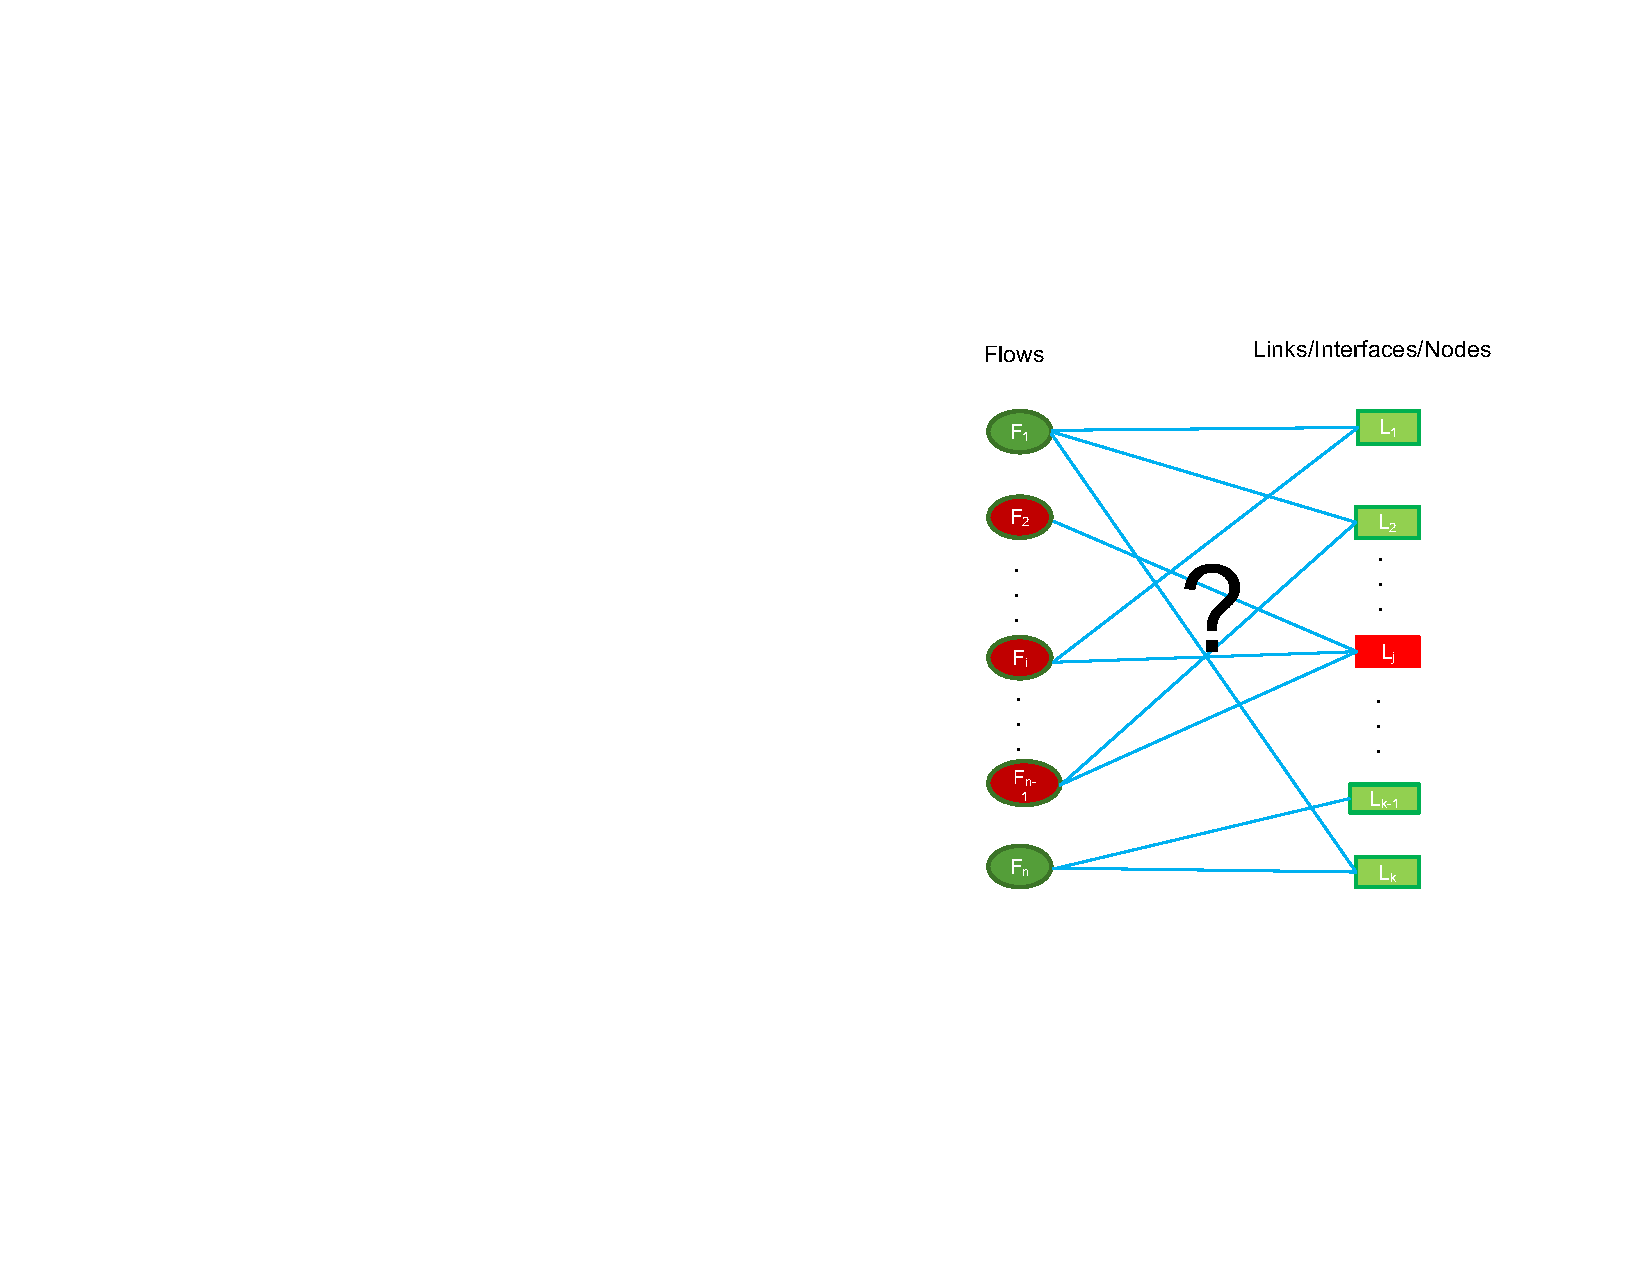
\includegraphics[width=0.25\textwidth]{./figure/RCABipartite}
  \end{center}
  \vspace{-5pt}
\caption{RCA Bipartite Graph}
\vspace{-5pt}
\label{fig:bipartite}
\end{wrapfigure}

The majority of recent work assume flow information between any pair of nodes in the network is available because they focus on data center networks that they have full ownership and modern routers allow originating and receiving probing data. This is very important because, as shown in~\cite{netbouncer:nsdi18}, there exists a minimal set of source-destination pairs to guarantee successful pinpointing of link errors in the network. Some of the work further assume they even know the routes for every flow, i.e., the mapping represented in Fig.~\ref{fig:bipartite}. However, both assumptions do not hold for our targeted multi-domain network environment due to obvious administrative constraints and the fact that, in the Internet scale network, traffic routing and forwarding are largely dynamically decided by the control plane software like OSPF and BGP subject to frequent topology and policy changes. 

We therefore made more restrictive but more realistic assumptions in this study in that (1) only the data file transfer information including integrity error states can be obtained at the end hosts from application layer; (2) only the physical nodes (domains) and their interfaces are known to us, but the network topology and traffic routing are unknown. 

In a large network, collecting the passive monitoring data from all node pairs may not scale well. Therefore, injecting probe packets between the designated node pairs periodically is adapted by several existing RCA systems. In practice, due to the probabilistic nature of the grey failures, controlled fault injection is an efficient way to generate training data within a reasonable time frame.

Directly accessing the production system to instrument the analysis with either active probing or fault injection is not realistic in most cases, especially in a multi-domain system where no one owns the entire infrastructure like in the data center networks. We believe emulation with realistic scales is a viable choice, given advanced Cloud testbeds are available.

